\usepackage[utf8]{inputenc}
 
\frenchspacing
\setlength{\parskip}{\baselineskip}%
 
 \usepackage{fancyhdr}
 \makeatletter
\renewcommand{\@chapapp}{Lecture}
\makeatother
 
 \usepackage{minitoc}
 
 %%
 \usepackage{placeins}
 
%% use enumlist for better control of 
\usepackage{enumitem}

\usepackage{array,multirow,graphicx}
%\usepackage{adjustbox}

%% use wrap figure package so that text can wrap around figures
\usepackage{wrapfig}
%\setlength{\intextsep}{-2pt}%
%% specify page geometry
\usepackage[margin=1.2in]{geometry}   
%\usepackage{showframe}
%% set up \href macro
\usepackage{hyperref}
\hypersetup{
    colorlinks=true,
    linkcolor=brown,
    filecolor=magenta,      
    urlcolor=blue,
}

%% SEE THIS LATER ON
%% https://www.latex4technics.com/?note=1np4
%% 

%% define some macros
\newcommand{\mytilde}{\raise.17ex\hbox{$\scriptstyle\sim$}}

\usepackage[usenames,dvipsnames,table]{xcolor}


\usepackage[breakable, theorems, skins]{tcolorbox}
\tcbset{enhanced}

\DeclareRobustCommand{\myvbox}[2][gray!20]{%
\vspace{8pt}\begin{tcolorbox}[   %% Adjust the following parameters at will.
        breakable,
        left=0pt,
        right=0pt,
        top=0pt,
        bottom=0pt,
        colback=#1,
        colframe=#1,
        width=\dimexpr\textwidth\relax, 
        enlarge left by=0mm,
        boxsep=5pt,
        arc=0pt,outer arc=0pt,
        ]
        \texttt{#2}
        \end{tcolorbox}
}

\newenvironment{tsession}[1]{%
\vspace{8pt}
\begin{tcolorbox}[breakable,
                  left=0pt,
                  right=0pt,
                  top=0pt,
                  bottom=0pt,
                  colback=#1,
                  colframe=#1,
                  width=\dimexpr\textwidth\relax,
                  enlarge left by=0mm,
                  boxsep=5pt,
                  arc=0pt,outer arc=0pt]
}{%
\end{tcolorbox}
}

%% author
% \author{Tim Warburton\vspace{12pt}\\with contributions from\vspace{8pt}\\ Anthony P. Austin \\ Andreas Kl"{o}ckner\\ Russell J. Hewett \\ Justin Krometis \\ Jonathan Baker}
%% author
\newcommand{\autha}{Ali Karakus}
\newcommand{\authb}{Tim Warburton}
\newcommand{\course}{Computational Science Foundations for Mechanical Engineers}
\newcommand{\code}{ME4XX}
\newcommand{\semester}{spring 2021}
\newcommand{\school}{Middle East Technical University}
\author{\autha{}  \& \authb{} \vspace{12pt}\\with contributions from\vspace{8pt}\\ Anthony Austin \\ Noel Chalmers \\Kasia \'{S}wirydowicz}

%% use today's date
\date{\today}

\newcommand{\VB}{VirtualBox}
\newcommand{\mytoc}{\dominitoc\renewcommand{\baselinestretch}{0.75}\normalsize \tableofcontents\renewcommand{\baselinestretch}{1.0}\normalsize\newpage}

\newcommand{\itemimage}[1]{ 
    \begin{center}
    \begin{minipage}[t]{0.8\textwidth}
        \fbox{\includegraphics[width=0.75\textwidth]{#1}}
    \end{minipage}
    \end{center}}
    
    
% \newcommand{\copyrightPage}{\newpage
% %\begin{fullwidth}
% ~\vfill
% \thispagestyle{empty}
% Copyright \copyright\ \the\year\ Tim Warburton

% \par\textsc{Published by Tim Warburton}

% \par These lecture notes are provided as a courtesy for Virginia Tech students attending CMDA 3634 and CMDA 1984 in Fall 2019. The notes should not be redistributed without permission of the author.

% \par\textit{First printing, \date{\today}}}

\newcommand{\copyrightPage}{\newpage
%\begin{fullwidth}
~\vfill
\thispagestyle{empty}
Copyright \copyright\ \the\year\ \autha{} \& \authb{}

\par\textsc{Published by \autha{} \& \authb{}}

\par These lecture notes are provided as a courtesy for \school{} students attending \code{} in \semester{}. Some parts of the lecture notes are taken from the lecture notes of CMDA 3634 and CMDA 1984 offered at Virginia Tech in Fall 2019 by the permission of the author, Tim Warburton. The notes should not be redistributed without permission of the authors.

\par\textit{First printing, \date{\today}}}

\usepackage{enumitem}

\newcommand{\boximage}[2]{
\begin{figure}[htbp!]
    \centering
    \fbox{\includegraphics[width=0.8\textwidth]{#1}}
    \caption{#2}
\end{figure}
}

\newcommand{\boximagelabel}[3]{
\begin{figure}[htbp!]
    \centering
    \fbox{\includegraphics[width=0.8\textwidth]{#1}}
    \caption{#2}
    \label{#3}
\end{figure}
}

%% quotes
\usepackage{epigraph}

\definecolor{mygreen}{rgb}{0,0.6,0}
\definecolor{mygray}{rgb}{0.95,0.95,0.95}
\definecolor{mymauve}{rgb}{0.58,0,0.82}
\definecolor{mycodebg}{rgb}{1,0.96,0.83}
\definecolor{mytermbg}{rgb}{0.79,0.99,0.96}
%\definecolor{mypythonbg}{rgb}{0.92,0.65,0.03}
\definecolor{mypythonbg}{rgb}{0.95,0.95,0.97}
\definecolor{myoutputbg}{rgb}{1.0,0.6, 0}
\definecolor{myexercise}{rgb}{0.52,0.80,0.98}
\definecolor{mymatlabbg}{rgb}{0.85,0.88,0.96}
% 255, 153, 0

%% source code listing
\usepackage{minted}

\setminted[c]{autogobble=true, frame=lines, framesep=4mm, baselinestretch=1.2, bgcolor=mycodebg, fontsize=\footnotesize,linenos=true}

\setminted[latex]{autogobble=true, frame=lines, framesep=4mm, baselinestretch=1.2, bgcolor=mygray, fontsize=\footnotesize,linenos=true}

\setminted[text]{autogobble=true, frame=lines, framesep=4mm, baselinestretch=1.2, bgcolor=mygray, fontsize=\footnotesize,linenos=false}

\setminted[python]{autogobble=true, frame=lines, framesep=4mm, baselinestretch=1.2, bgcolor=mycodebg, fontsize=\footnotesize,linenos=true}

\setminted[bash]{autogobble=true, frame=lines, framesep=4mm, baselinestretch=1.2, bgcolor=mygray, fontsize=\footnotesize,linenos=true}

\setminted[R]{autogobble=true, frame=lines, framesep=4mm, baselinestretch=1.2, bgcolor=mycodebg, fontsize=\footnotesize,linenos=true}

\setminted[matlab]{autogobble=true, frame=lines, framesep=4mm, baselinestretch=1.2, bgcolor=mymatlabbg, fontsize=\footnotesize,linenos=true}


\usepackage{multicol}
\usepackage{amssymb}
\usepackage{amsmath}

\DeclareMathOperator*{\argmax}{arg\,max}
\DeclareMathOperator*{\argmin}{arg\,min}

\usepackage[normalem]{ulem}

\usepackage[ruled,vlined,commentsnumbered]{algorithm2e}

\SetKwInput{KwInput}{Input}
\SetKwInput{KwOutput}{Output}
\SetKwInput{KwInputOutput}{Input/Output}
\SetKwInput{KwRequire}{Require}

%% add horizontal rule for algorithms
%% (http://tex.stackexchange.com/questions/52456/horizontal-line-in-algorithmic-environment)
\makeatletter
\newcommand{\algrule}[1][.2pt]{\par\vskip.5\baselineskip\hrule height #1\par\vskip.5\baselineskip}
\makeatother

% Comment the following to have chapters numbered without interruption (numbering through parts)
%\makeatletter\@addtoreset{chapter}{part}\makeatother%

\usepackage[sorting=none, backend=biber, refsection = chapter]{biblatex} 

\addbibresource{me4xx.bib}

\usepackage{pgf,tikz}
\usepackage{pgfplots}


\makeatletter
\newcommand{\chapterauthor}[1]{%
  {\parindent0pt\vspace*{-25pt}%
  \linespread{1.1}\large\scshape#1%
  \par\nobreak\vspace*{25pt}}
  \@afterheading%
}
\makeatother

%\usepackage{titlepic}
%\titlepic{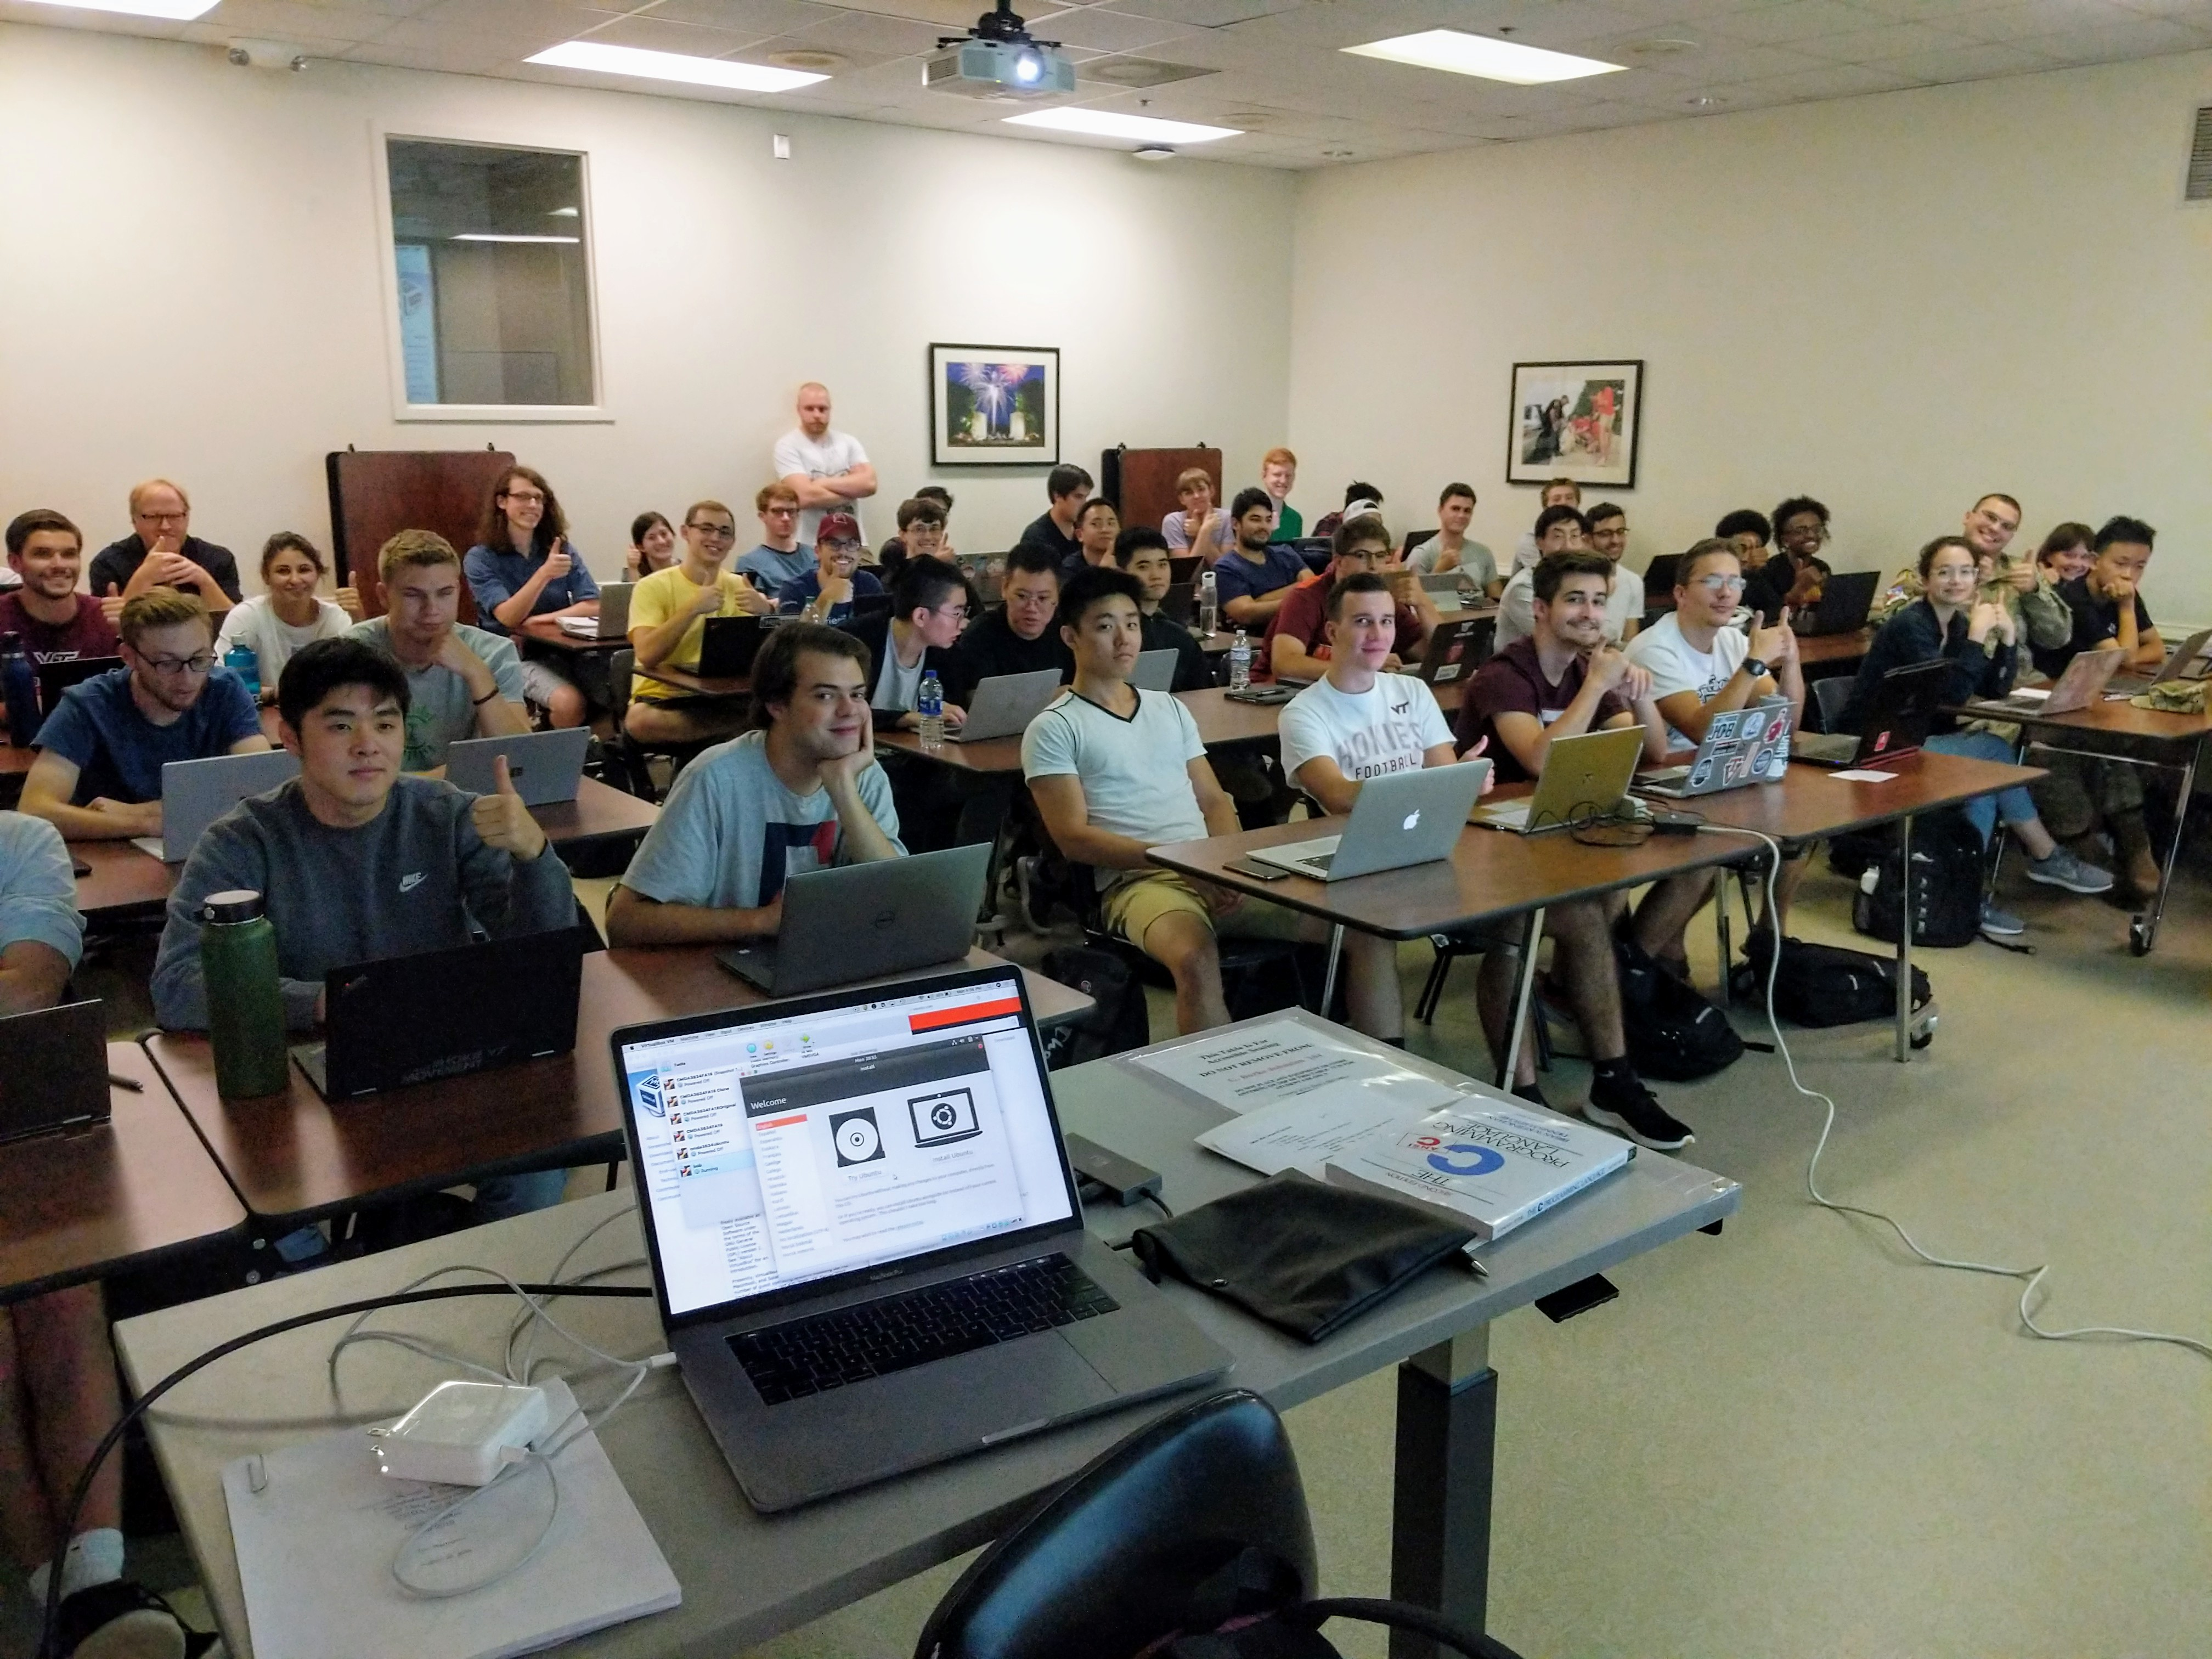
\includegraphics[width=\textwidth]{figures/cover/IMG_20190826_165553.jpg}}
\usepackage{fix-cm}
\newcommand{\bigsize}{\fontsize{35pt}{20pt}\selectfont}

\newcommand{\mycall}[2]{\textcolor{#1}{#2}}

\usepackage{exercise,chngcntr}
\counterwithin{Exercise}{chapter}
\counterwithin{Answer}{chapter}

\renewcommand{\ExerciseHeader}{%
  \par\noindent
  \textbf{\large \ExerciseName{} \ExerciseHeaderNB{}\ExerciseHeaderTitle{}\ExerciseHeaderOrigin}%
  \par\nopagebreak\medskip
}

\renewcommand{\AnswerHeader}{%
  \par\noindent
  \textbf{\large \AnswerName{} \ExerciseHeaderNB{}\ExerciseHeaderTitle{}}%
  \par\nopagebreak\medskip
}

%% for movies
\usepackage{media9}

\newcommand{\myparagraph}[1]{{\bf #1}:}
\newcommand{\myquote}[1]{\vspace{2pt}{``\emph{#1}''}\vspace{2pt}}

%% source of thumbs up
%% https://fontawesome.com/icons?d=gallery&q=thumbs
\usepackage{fontawesome}

\usepackage{comment}

\usepackage[font=small,labelfont=bf]{caption}

\newcommand{\tbs}{\textbackslash}
\usepackage{amsmath}
\usepackage{amsfonts}
\usepackage{amssymb}
\usepackage{amsthm}
\newtheorem{thm}{Theorem}

\usepackage{longtable}
\usepackage{array,etoolbox}
\preto\tabular{\setcounter{magicrownumbers}{0}}
\newcounter{magicrownumbers}
\def\rownumber{}
